\section{Background Theory}
\iffalse
\begin{itemize}
    \item Husk rød tråd.
    \item Vær generisk.
    \item Bare inkluder konsept som blir relevante senere, eller som er brukt i nødvendige antagelser.
    \item many of the concepts explained in this chapter were also explained in [TODO: fordypningsprosjekt].
    \item The goal of this chapter is to explain all the concepts neccessary to understand how the trajeoctyr planning algorithm works.
    Additionally, it should grant an understanding as to why the algorithm ended up the way it is.
\end{itemize}
\fi
This chapter will introduce the concepts and theory neccessary to understand the design and intent behind the trajectoy planning algorithm, as well as the discussion on it's functionality.
The goal of the chapter is that the reader will have enough intuition of the applied theory that the proposed arguments and solutions should make sense. In addition, the chapter is structured
so that it should be easy to quickly navigate and read about specific topics.
\subsection{Vessel modelling}
\iffalse
--------- Genereal thoughts --------------------------

Jeg tenker det er best å skrive om modellering i sammenheng med hvordan trajectory planning problemet blir satt opp i MATLAB med CasADi.
\begin{itemize}
    \item Kinematics \& Kinetics -\> Begge brukes i CasADi setup.
    %\item Munk moment -> Potensielt relevant hvis jeg skriver om modellerings problemer
    \item Her kan det også skrives om de spesifike tallverdiene som blir brukt i Masse, coriolis og dempnings -matrisene.
    de er spesifike til Milliampere, funnet gjennom en rekke forsøk utfort av Anders Pedersen.
\end{itemize}
---------- /General Thoughts--------------------------- 
\fi
\begin{figure}
    \centering
    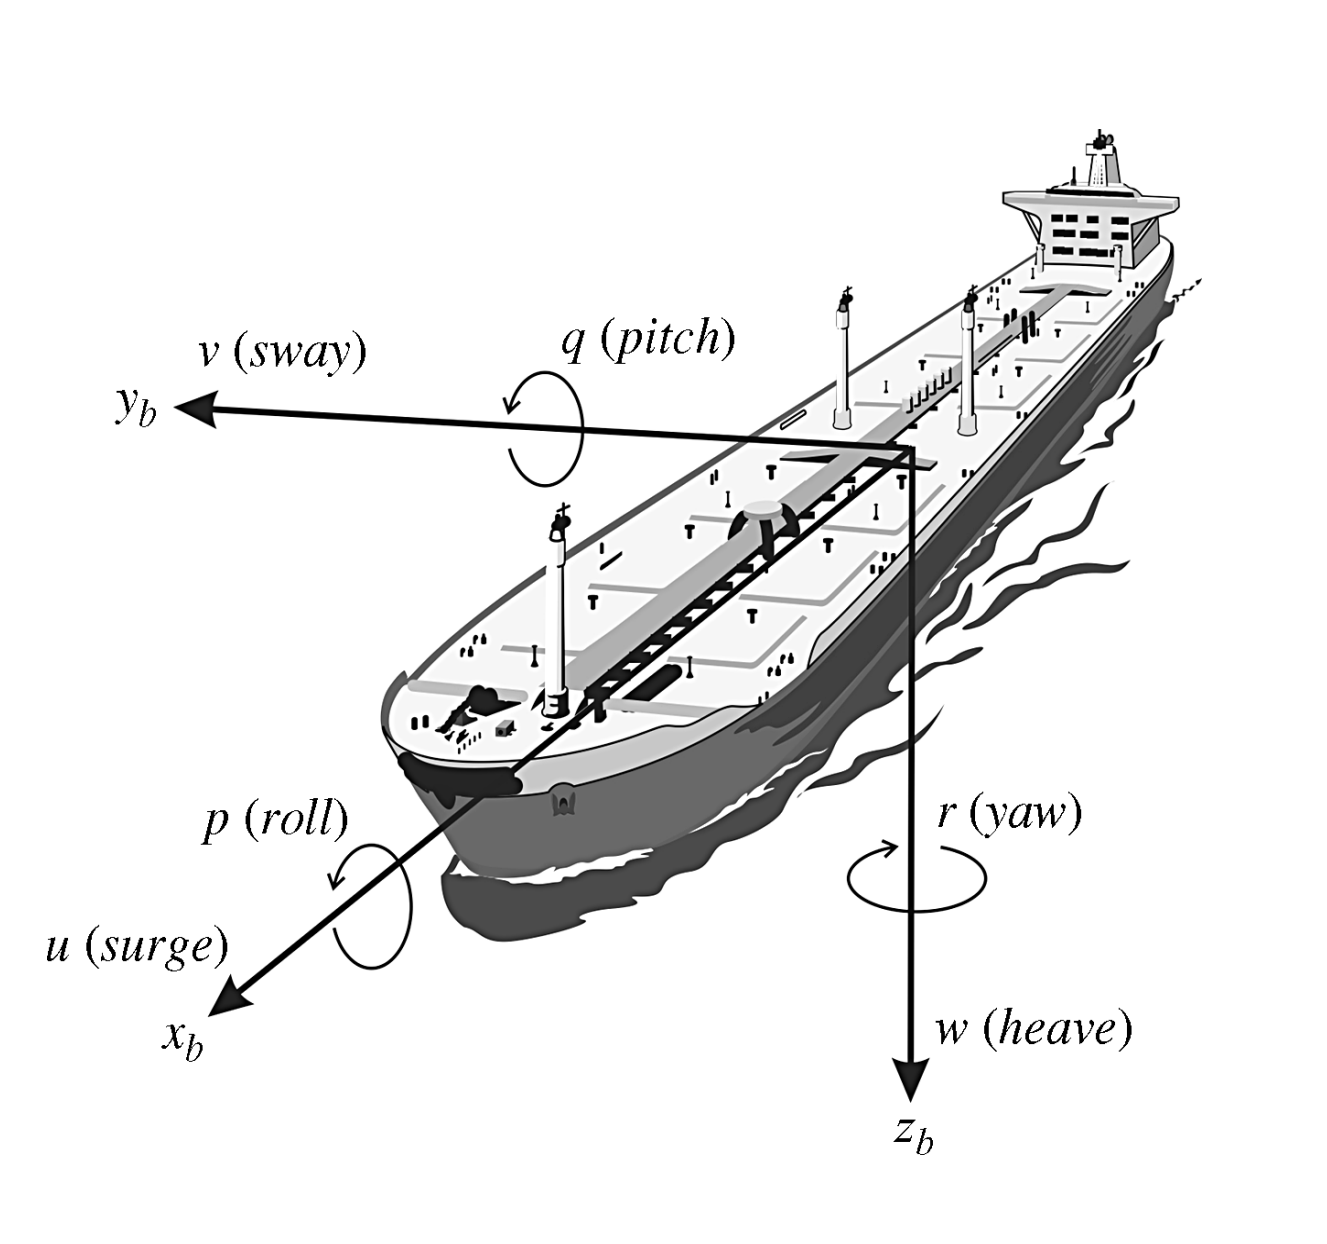
\includegraphics[height=0.35\textheight]{Images/SHIPDOF_FOSSEN.png}
    \caption{A ships 6 degrees of Freedom, from \cite{fossen2011handbook}}
    \label{FIG: Ship DOF}
\end{figure}
\iffalse
\begin{itemize}
    \item A model in this context is just a way of describing how physical systems change over time.
    \item There are many different ways to make models, and different models are suitable for modelling different aspects of the physical world.
    \item The model described in this chapter, and used for the thesis, is a 3 \gls{DOF} nonlinear model based on the work of \cite{fossen2011handbook}.
    \item The model can also incorporate wind and current disturbances, but they are omitted from this thesis.
    \item The parameter values will vary from ship to ship, this thesis will operate with numbers for the NTNU milliampere ferry.
    the parameters were found through testing by \cite{andersson2019casadi}
    \item pose is parameterized in the \gls{NED} coordinate frame where the 
\end{itemize}
\fi
% A mathematical model is a tool for describing physical systems and expressing how they change over time, models are not unique and there are many different ways of modelling a physical system, they all have strengths and weaknesses.
% % The model applied in this thesis is based on the theory and notation by \cite{fossen2011handbook},

A mathematical model is a tool for describing physical systems and expressing how they change over time, respond to external forces, and how stable the system might be. Models are very useful when designing control systems as
they translate the physical into equations that computers can understand. When making a model it is often useful to seperate the dynamics of the different parts of the 
system we are interested in, these are the \gls{DOF} the system has, and is often the directions the system can move, though they can also just be
nondescript generalized coordinates. Deciding which \gls{DOF} to seperate out and model the dynamics of is often what seperates models from each other, it is pointless to model
an aspect of a system that there is no intent to interact with. For example a ship has six \gls{DOF}, see Figure \ref{FIG: Ship DOF}, for modelling a control system for stationkeeping
all six are important because stationkeeping involves keeping the whole ship as steady as possible. When modelling for path following on the other hand it is not
important what the heave, roll, or pitch of our vessel is and so the dynamics of those \gls{DOF} can safely be ignored. 
The model used to describe our vessel in this thesis is based on the theory and notation by \cite{fossen2011handbook}, and is a 3\gls{DOF} nonlinear mass-damper system with
thruster dynamics and no external disturbances such as wind or currents. The dynamics of the vessel can be described by the differential equations below:

\begin{equation} \label{EQ: eta_dot}
    \bm{\dot{\eta}} = \textbf{R}(\psi)\bm{\nu}    
\end{equation}
\begin{equation} \label{EQ: Vessel Dynamics}
    \textbf{M}\bm{\dot{\nu}} + \textbf{C}(\bm{\nu})\bm{\nu} + \textbf{D}(\bm{\nu})\bm{\nu} = \bm{\tau}
\end{equation}

Where $\bm{\eta}$ is the pose of the vessel, parameterized in the tangental plane \gls{NED} where the x-axis points towards true north, the y-axis east and the z-axis down towards the center of the planet.
The \gls{NED} frame can be said to be inertial for short distance control objectives.
The vector $\bm{\eta}$ is a column vector with the vessel's North, East and Heading values, which are the three \gls{DOF} of the system. The $\bm{\nu}$ vector is a column vector containing
the vessel's velocities parameterized in the BODY frame, namely surge, sway, and yaw rate. In the BODY frame there are no fixed rules for where the axis are pointing, but the common convention for modelling
vehicles is that the x-axis points along the lognitudal axis of the vessel, the y-axis points along the lateral axis and the z-axis points along the vertical axis. This is also seen in Figure \ref{FIG: Ship DOF}.
The anchor point for the BODY frame is arbitrary but always fixed to the vessel and moves with it. \textbf{R} is a rotational matrix about the heading ($\psi$) of the vessel and it transform the BODY velocities into
NED movement. 
The Rotation matrix, as well as pose, velocity, and the thruster vector $\bm{\tau}$ are:

\begin{equation}
    \textbf{R}(\psi) = \begin{bmatrix}
                        cos\psi &   -sin\psi & 0\\[-5pt]
                        sin\psi & cos\psi    & 0\\[-5pt]
                        0       &   0        & 1
                        \end{bmatrix}
\end{equation}
\begin{equation}
    \bm{\eta} = \begin{bmatrix}
                x   &    y  &    \psi
                \end{bmatrix}^T
\end{equation}
\begin{equation}
    \bm{\nu} = \begin{bmatrix}
                 u   &   v  &    r
                \end{bmatrix}^T
\end{equation}
\begin{equation} \label{EQ: Tau}
    \bm{\tau} = \begin{bmatrix}
                F_{X}   &   F_{Y}  &   F_{N}
                \end{bmatrix}^T
\end{equation}
\iffalse
\begin{itemize}
    \item $\eta$ is defined in the \gls{NED} reference frame, $\nu$ is defined in BODY frame, briefly explain what that means.
    \item The M and C matrices are a combination of Rigid body and hydrodynamic added mass matrices
    \item Fully computing the M and C matrices is a lot of work, for milliampere the work has already been conducted
    by Andreas Pedersen.
    \item If the model values are to be found through experiementation it's senseless to seperate Rigid body and hydrodynamic added mass.
    The matrices then become:
\end{itemize}
\fi

In \ref{EQ: Vessel Dynamics} the \textbf{M} matrix is the inertia matrix of the system, which describes how 'heavy' the \gls{DOF} are to nudge, in
addition to the vessel's inherent inertia from being massive the vessel must also push water out of the way when it moves, this is what is known as
hydrodynamic added mass and is linearly added to the inertia matrix. The coriolis matrix \textbf{C} also has to include hydrodynamic added mass,
however for the purpose of this thesis it is not important to know the parameters for either of these matrices or for the dampening matrix \textbf{D}.
That is because a trajectory planning algorithm needs to work regardless of vessel parameters, \cite{pedersen2019optimization} explains more in-depth
how the system parameters can be found. Continuing on, the dampening matrix is a linear combination of the linear dampening stemming from water
viscosity and non-linear dampening from cross-flow, once again the parameters themselves are not strictly relevant to this thesis, but intuition is
important. The result are matrices in the following form:

\begin{equation}
    \textbf{M} = \begin{bmatrix}
                m11 &   m12 &   m13\\[-5pt]
                m12 &   m22 &   m23\\[-5pt]
                m31 &   m32 &   m33
                 \end{bmatrix}
\end{equation}

\begin{equation}
    \textbf{C}(\bm{\nu}) =  \begin{bmatrix}
        0             &     0       &   c13(\bm{\nu})\\[-5pt]
        0             &     0       &   c23(\bm{\nu})\\[-5pt]
        c31(\bm{\nu}) &c32(\bm{\nu})&   0
                            \end{bmatrix}    
\end{equation}

\begin{equation}
    \textbf{D}(\bm{\nu}) =  \begin{bmatrix}
        d11(\bm{\nu}) &     0       &   0\\[-5pt]
        0             &d22(\bm{\nu})&d23(\bm{\nu})\\[-5pt]
        0             &d32(\bm{\nu})&d33(\bm{\nu})
                            \end{bmatrix}       
\end{equation}

The dampening matrix can be a bit of a compuational nightmare and can be simplified to a linear and diagonal matrix without too much
of a detrimental impact on our simulations. The justification for this simplification is the underlying assumption that the reference output
from the trajectory planner algorithm will be parsed through a final control module that will account for dampening. The risk is that
the end result from the trajectory planner turns out to be infeasible, but that's a problem for another thesis.

\begin{equation}
    \textbf{D}(\bm{\nu}) = \begin{bmatrix}
                            d11 &   0   &   0\\[-5pt]
                            0   &   d22 &   0\\[-5pt]
                            0   &   0   &   d33
                            \end{bmatrix}
\end{equation}

Finally, a word on heading vs course. Throughout this thesis the terms course and heading might be used interchangeably, but the words are strictly not synonymous.
Heading is equivalent with yaw as both denote a rotation about the vessel's third axis, the difference between the two is that yaw is often a relative term describing
a change by some degrees from one arbitrary pose to another. Heading is an absolute term and is often based on compass directions, meaning 0\textdegree heading
equates to the nose of the vessel pointing towards true north. Neither heading nor yaw is equivalent with course, which is strictly the direction
of travel relative to true north. In a simplified world void of disturbances heading and course will align during straight line
travel, but external forces such as wind or currents will cause the two angles to deviate. Likevise sideslip caused by a non-zero sway velocity when turning will 
also introduce a deviation between course and heading(TODO: Citation needed?). However this difference is mostly unrelated to the work put forth in this thesis, 
and so the terms heading and course might be used interchangeably. Althought it often makes sense to deliberately pick one
term over the other.


\subsection{Trajectory Planning}
\iffalse
--------- Genereal thoughts --------------------------
\begin{itemize}
    \item How to get from A to B.
    \item Multiple methods, all with pros and cons, skriv liten oversikt.
    \subitem LOS, OCP, Machine Learning, osv.
    \subitem Kanskje ikke så veldig viktig å snakke om andre metoder enn OCP.  
    \item Important factors to consider:
    \subitem Time horizon / length of planning period.
    \subitem Trajectory safety with respect to ship capabilities.
    \subitem \gls{COLREGs} compliance 
    with respect to expected behaviour.
    \subitem osv.
    \item Litt dypere inn i numerisk optimalisering og MPC, og LOS ettersom det kommer til å bli brukt igjen senere.
    \item Disambiguate Path vs Trajectory
   % \item Først oversikt, deretter enten nytt kapittel eller delkapittel om 
   % den spesifikke metoden jeg skal bruke, forklar numerisk optimalisering, MPC, LOS guidance, hvordan alt kombineres til å bli min algoritme, in theory.
\end{itemize}
--------- /Genereal thoughts --------------------------
\fi

% \begin{itemize}
%     \item Core concept. Path VS Trajectory.
%     \item Many ways of doing it.
%     \item chosen method for this thesis.
%     \item Numerical optimization, OCP, NLP, MPC.
% \end{itemize}

% Because the model for describing the dynamics of our vessel is a set of ordinary differential equations we can solve them for the input we need
% to achieve any desired state. And because the dynamics are time-invariant we can solve for any future time interval given initial conditions.
Because the vessel dynamics are described by a model expressed as a set of time-invariant ordinary differential equations, any desired state
can be reached by solving for the sequence of inputs that will take the vessel from a given initial condition to said state. In the context of this
thesis "state" refers to the pose, $\bm{\eta}$, of the vessel. The simplest application of this would be moving in a straight line from point A to point B.
The solution is simply to find the input sequence which turns the vessel to the correct course and then maintaining a forward speed until point B is reached.
The straight vector line from point A to point B can be thought of as the desired or reference path, while the sequence of states achieved by applying the 
input sequence is the trajectory. Instead of having just one destination there might be multiple waypoints forming the path, and the optimal
input sequence that makes the vessel travel along the path depends on what criteria are considered important. A trajectory generated with fuel
economy in mind might look very different from a trajectory generated with shortest transit time in mind, even if both are following the same path.
Other factors such as obstacles or disturbances will also influence the trajectory, combining all the factors and generating the desired
input sequence is the act of trajectory planning.

There are many methods for trajectory planning. Some are conceptually simple and fast to compute, but lack robustness and situational adaptability.
Or the method can be incredibly complex and and computationally involved, but in return incredibly robust to disturbances and adaptable to
any situation. An example of a simple trajectory planner would be a \gls{LOS} guidance law while something extremely advanced would be training a deep
neural network. For an overview: in this thesis a \gls{LOS} guidance law will be applied to generate a reference trajectory, the reference is then used as part of a
formulation of an \gls{OCP} with a cost to penalize deviation from the reference in addition to other factors. The \gls{OCP} is then discretized
as a \gls{NLP} problem using a method called direct multiple shooting, finally the \gls{NLP} is solved with an \gls{IPOPT} solver.

\subsubsection*{Line of Sight Guidance}
% \begin{itemize}
%     \item Path following algorithm.
%     \item Cross track and along track errors.
%     \item integral action.
%     \item course control will not be neccessary.
%     \item Only considering the horizontal control.
%     \item Suppressing cross track error towards zero gives the desirec course to follow.
%     \item When the along track error is below a certain threshold k = k + 1 (move to the next waypoint)
%     \item \cite{lekkas2013line}
% \end{itemize}

This guidance method is perhaps the most intuitive; consider the waypoints WP\textsubscript{k} and WP\textsubscript{k+1}, the simplest path
from one to the other would be straight line. Therefor the most obvious control method would be to maneuver onto the straight line, and
follow it along to the end. The distance of the controlled vessel to the straight line is called the cross track error $y_e$ and the distance along the line
to the end is called the along track error $x_e$. The along track error is not of any importance to this thesis, it is assumed that the controlled
vessel will maintain a steady velocity, and there are no temporal constraints on reaching the goal.

As explained in \cite{lekkas2013line}; given the controlled vessel's position (x,y), the cross track and along track errors from the straigth line as defined by WP\textsubscript{k} (x\textsubscript{k},y\textsubscript{k})
and WP\textsubscript{k+1} (x\textsubscript{k+1}, y\textsubscript{k+1}) are:
\begin{equation} %% Along track and Cross Track error
    \begin{bmatrix}
        x_e \\[-5pt]
         ye
    \end{bmatrix} = \textbf{R}^T(\gamma_p) \begin{bmatrix}
                                            x - x_k \\[-5pt]
                                            y - y_k
                                            \end{bmatrix}
\end{equation}
Where R is the rotation matrix from the inetiral frame to the straight line's frame. $\gamma_p$ is the horizontal path-tangental angle,
or the 'angle' of the straight line path in relation to the inetrial frame if that makes more sense. The rotation matrix \textbf{R} is given by:
\begin{equation} %% Rotation matrix R(gamma)
    \textbf{R}(\gamma_p) = \begin{bmatrix}
                            cos(\gamma_p) & -sin(\gamma_p) \\[-5pt]
                            sin(\gamma_p) & cos(\gamma_p)
                            \end{bmatrix}
\end{equation}
with $\gamma_p$:
\begin{equation} %% Calculating Gamma
    \gamma_p = \textrm{atan2}(y_{k+1} - y_k , x_{k+1} - x_k)
\end{equation}
The control objective is to drive $y_{e}(t) \rightarrow 0.$ as t trends towards infinity. Assuming a steady velocity this is done by
selecting a course that steers the controlled vessel in the direction that reduces $y_e$. How fast the error $y_e$ is suppressed is
tuned by a proportional gain factor, $\varDelta$, that is often called look ahead distance. The desired heading is given by:
\begin{equation} %% Calculating psi_d
    \psi_d = \gamma_p + \arctan(\frac{-y_e}{\varDelta})
\end{equation}
and consequently desired course:
\begin{equation}
    \chi_d = \psi_d + \beta
\end{equation}
Where $\beta$ is the sideslip of the controlled vessel. Because real life situations are rarely, if ever, devoid of disturbances that introduce
sideslip and crab angles there is one common improvement that can be made: Integrate the cross track error and use both current cross track error
and it's integral when calculating desired heading. The equation for $\dot{y}_{int}$ and $\psi_d$ then become:
\begin{equation}
    \dot{y}_{int} = y_e
\end{equation}
\begin{equation}
    \psi_d = \gamma_p - \arctan(K_{p}y_e + K_{i}\dot{y}_{int})
\end{equation}
Where K\textsubscript{p} and K\textsubscript{i} are gain parameters proportional to the lookahead distance, typically $K_p = (1/\varDelta)$, $K_i = Kp*\kappa$
with $\kappa > 0$ being some design variable.

A reference trajectory is generated by using the LOS law as described to guide the \gls{OS} from it's initial position through all the waypoints, and
saving the desired positions and velocities after each time step. For a path with more than two waypoints a simple index incrementation can be used when the
\gls{OS} is within a certain distance from it's current target waypoint. The reference trajectory from $t_0$ to N iterations of \gls{LOS} applications is of the form:
\begin{subequations}
    \begin{align}
        \overline{\bm{\eta}}_{ref} \quad & = [\bm{\eta}_{t0} \ , \ \bm{\eta}_{t+1} \ , \ \dots \ , \bm{\eta}_N] \\ 
        \overline{\bm{\nu}}_{ref} \quad & = [\bm{\nu}_{t0} \ , \ \bm{\nu}_{t+1} \ , \ \dots \ , \bm{\nu}_N]
    \end{align}
\end{subequations}

\subsubsection*{Optimal Control Problem}
% \begin{itemize}
%     \item Equations.
%     \item Model Predictive Control is simulating the dynamics of the system with a desired control objective and then applying the first states as
%     reference for the vessel's control system. After actuation new measurements are taken and the model is simulated again from the new initial conditions.
%     \item Many ways to solve an optimization problem, often quite difficult due to Continuous dynamics.
%     \item cite \cite{breivik2017mpc} for a quick look and equation formulation.
%     \item cite \cite{wright1999numerical} For a comprehensive lesson on optimal control.
% \end{itemize}
Numerical optimization is a vast field within mathematics, \cite{wright1999numerical} explains it well: There are no universal optimization algorithm. Instead an algorithm must be tailored to the optimization
problem. Within the context of trajectory planning there are different parameters to optimize for, some examples are: maintaining steady velocity, suppressing sway, minimalizing
fuel waste, minimizing distance to goal, and there are many more. The general expression for an optimization problem can be written as simple as:
\begin{subequations}
    \begin{align}
    \underset{x\in \textbf{R}^n}{\textrm{Minimize}} \quad & f(x) \\
        \textrm{Subject to:} \quad & c_i(x) = 0, \quad i \in \mathcal{E} \\
                             \quad & c_i(x) \geq 0, \quad i \in \mathcal{I} 
    \end{align}
\end{subequations}
% \begin{itemize}
%     \item However a better generalized formulation was made in \cite{breivik2017mpc}, it's basically the same but expressed in a way that will be easier to use later.
%     \item The cost function is 
% \end{itemize}
Where $f(x)$ is some continuous function, $c_i$ are constraint functions on the system which $f(x)$ exists in, and $\mathcal{E}$ and $\mathcal{I}$ are indices
pertaining to if the constraint $c_i$ is an equality or inequality constraint. In the context of this thesis the thing to minimize is some nebulous cost function
associated with path following, and the constraints are the physical model of the system that guarantees feasibility as well as safety constraints to avoid collisions.
The cost function is then some function of the vessel's state, reference trajectory, and control input. The two constraints are the system dynamics from \ref{EQ: Vessel Dynamics}
and \ref{EQ: eta_dot}. And then additional constraints for collision safety and initial conditions. A new general \gls{OCP} definition is thus given by the following:

\begin{subequations}
    \label{EQ :OCP description}
\begin{align}
    % \textrm{Minimize} \quad & \textbf{F}(\boldsymbol{\eta}(t), \textbf{u}(t)) \label{eq:OCP-a} \\ 
    % \textrm{subject to} \quad & \dot{\boldsymbol{\eta}}(t) = \textbf{L}(\boldsymbol{\eta}(t), \textbf{u}(t)) \label{eq:OCP-b} \\
    % \quad & \textbf{h}(\boldsymbol{\eta}(t), \textbf{u}(t)) \leq \textbf{0} \label{eq:OCP-c}\\
    % \quad & \boldsymbol{\eta}(t_0) = \boldsymbol{\eta}_0 \label{eq:OCP-d}
    \textrm{Minimize} \quad & {L}(\bm{\theta}(t), \bm{\theta}_{ref}(t), \bm{\tau}(t)) \\
    \textrm{Subject to:} \quad & \dot{\bm{\theta}}(t) = \textbf{J}(\bm{\theta}, \bm{\tau}) \\
                         \quad & \textbf{h}(\bm{\theta}(t), \bm{\tau}(t)) \leq 0 \\
                         \quad & \bm{\theta}(t_0) - \overline{\bm{\theta}}_0 = 0
\end{align}
\end{subequations}
where L is the cost function, $\bm{\theta} = [\bm{\eta}^T \ , \ \bm{\nu}^T]^T$ and $\bm{\tau}$ is the same as in \ref{EQ: Tau}. 
\textbf{J}($\bm{\theta}, \bm{\tau}$) Are the model dynamics \ref{EQ: eta_dot}, \ref{EQ: Vessel Dynamics}. $\overline{\bm{\theta}}_0$ are the
given intial conditions of the system.
The solution to the optimization problem is the series of inputs $\bm{\tau}$ which minimizes the integral of the cost L 
from t\textsubscript{0} to t\textsubscript{end}. And L has the form of a quadratic function
akin to a weighted least squares: (TODO: Eh, grei formulering?)
\begin{equation}
    L(\bm{\theta}(t), \bm{\theta}_{ref}(t), \bm{\tau}(t)) = (\bm{\theta}(t) - \bm{\theta}_{ref}(t))^T \textbf{Q} (\bm{\theta}(t) - \bm{\theta}_{ref}(t)) + \textbf{K}_\tau \bm{\tau}^2
\end{equation}
Where the diagonal of the \textbf{Q} matrix are the weight coefficients of deviating from the reference
and \textbf{K}\textsubscript{$\tau$} denote the associated cost of applying force in the three \gls{DOF}.

Solving the \gls{OCP} can be done using a multitude of methods, \cite{breivik2017mpc} suggest discretizing 
the \gls{OCP} into a \gls{NLP} using a method called direct multiple shooting.


\subsubsection*{NonLinear Programming}
% \begin{itemize}
%     \item discretized formulation of the OCP, using among many methods, Direct Multiple shooting.
%     \item I don't really understand this stuff too much.
%     \item Direct Multiple Shooting explanation needed.
%     \item shooting gaps.
%     \item cite \cite{gros2017Lecture} for direct multiple shooting
%     \item cite \cite{andersson2019casadi} Casadi for constructing the NLP in a 
%     computer friendly way, and \cite{wachter2006implementation} for IPOPT
% \end{itemize}
% \begin{itemize}
%     \item Direct multiple shooting is a discretized formulation of the \gls{OCP} where both the states and the control
%     inputs are explicitly defined as decision variables.
%     \item Because direct multiple shooting means the selected solver is 'free' to place the states and inputs wherever it wants
%     we must employ shooting constraints to enforce a physically feasible trajectory. This is called closing the shooting gaps.
%     \item A solver is an algorithm decined to crunch the NLP problem, 
%     in this thesis we will use an \gls{IPOPT} solver \cite{wachter2006implementation}.
%     \item To help formulate the \gls{NLP} a framework provided by \cite{andersson2019casadi} will be used.
%     \item The shooting gaps constraints are created by integrating forward one time step at each control interval
%     with a RK4 mehtod, which gives us a discret value $\omega$\textsubscript{k+1} using the continuous function $\textbf{f}(\bm{\omega})$. 
%     For each control interval k there must be a shooting gap constraint $\textbf{F}(\bm{\omega}_k) - \bm{\omega}_{k+1} = 0$. 
%     These shooting gap constraints are placed in \textbf{g}($\bm{\omega}$)
%     \item To avoid collisions constraints pertaining to illegal positions are also placed in \textbf{g}($\bm{\omega}$)
%     \item To make sure decision variables that are outside of 'legal' limits aren't searched for; The decision variables $\bm{\omega}$ are constrained by
%     upper and lower bounds which limits the search space with an upper and lower bound. 
%     This doesn't matter much for decision variables that are states, but matters a lot for velocities. ???
% \end{itemize}
The author would like to note that the technique used in this section, direct multiple shooting, is outside the scope of the author's knowledge.
Everything the author knows about this technique was learned over the course of the master thesis project, and it's highly recommended to read the full formulation by \cite{breivik2017mpc}
which is the formulation that the implementation for this thesis heavily builds upon. Another great resource for direct multiple shooting are the video lectures of \cite{gros2017Lecture}.
Also note that functions and definitions from the previous section on \gls{OCP} carry over, for example $\bm{\theta} = [\bm{\eta}^T \ , \ \bm{\nu}^T]^T$ still holds.\newline
Direct multiple shooting is a \gls{OCP} discretization technique where both the states and control inputs are excplicitly defined as decision variables.
The \gls{NLP} is then a reformulation of \ref{EQ :OCP description} where L is redefined as a discretized cost function with $N_p$ control intervals steps:
\begin{equation} %(TODO: GÅ GJENNOM DETTE)
    \Phi(\bm{\omega}, \bm{\omega}_{ref_{1:N_p}}) = 
    \sum_{k=0}^{N_{p}-1} ((\bm{\theta}_{k+1} - \bm{\theta}_{ref_{k+1}})^T Q (\bm{\theta}_{k+1} - \bm{\theta}_{ref_{k+1}}) + K_{\bm{\tau}} \bm{\tau_k}^2)
\end{equation}
where $\bm{\omega} = [\bm{\theta}_0^T \ , \ \bm{\tau}_0^T \ , \ ... \ , \ \bm{\theta}_{N_{p-1}}^T \ , \ \bm{\tau}_{N_{p-1}}^T \ , \ \bm{\theta}_{N_{p}}^T]^T \in \mathbb{R}^{9N_{p}+6}$
is a vector containing $5N_p + 6$ decision variables.% and $\bm{\theta}$ is the same as it was in \ref{EQ :OCP description}.
Because $\bm{\tau}_k$ does not have an accociated reference in this thesis; it is seperated out as it's own part of the function.
\textbf{Q} is still a sparse 6x6 matrix where the diagonal contain the tuning parameters,
and \textbf{K}\textsubscript{$\bm{\tau}$} are still tuning parameters on control input. The complete NLP will end up in the form of:
\begin{subequations}
    \label{EQ:NLP}
    \begin{align}
        % \min_{\boldsymbol{\omega}} \quad & \textbf{L}(\boldsymbol{\omega}) \label{eq:NLP-1} \\
        % \textrm{subject to} \quad & \boldsymbol{\omega}_{lb} \leq \boldsymbol{\omega} \leq \boldsymbol{\omega}_{ub} \\ 
        % \quad & \textbf{g}_{lb} \leq \textbf{g} \leq \textbf{g}_{ub}
        \min_{\bm{\omega}} \quad & \bm{\Phi}(\bm{\omega}, \bm{\omega}_{ref_{1:N_p}}) \\ %% (TODO: er det rett å ha min_w?)
        \textrm{Subject to:} \quad & \bm{\omega}_{lb} \leq \bm{\omega} \leq \bm{\omega}_{ub} \\
                            \quad & \textbf{g}(\bm{\omega})_{lb} \leq \textbf{g}(\bm{\omega}) \leq \textbf{g}(\bm{\omega})_{ub}
    \end{align}
\end{subequations}
where $\bm{\omega}_{lb}$ and $\bm{\omega}_{ub}$ are the lower and upper bounds on the permitted values for $\bm{\omega}$, this is meant to reduce the space searched when
solving the NLP, as well as limit the decision variables to physically feasible values. \textbf{g}($\bm{\omega}$) is a vector of constraint functions that are similarly bound
by an lower and upper bounds, where the bounds define if any given function in \textbf{g} is an equality or inequality constraint. Due to the way direct multiple shooting
defines the decision variables the programmed solver that solves the \gls{NLP} is free to place the states and velocities anywhere within the constraints. It is therefor
important to implement equality constraints that force the ending of one control interval and the beginning of the next to line up. this is called closing the shooting gaps, 
an illustration of what shooting gaps are can be seen in Figure \ref{FIG: Shooting Gaps}. These equality constraints are called shooting constraints and to create them begin
by defining an integrator function $\textbf{F}(\bm{\theta}_{k}, \bm{\tau}_k)$ using any technique, in this thesis the following \gls{RK4} method will be used:

\begin{figure}
    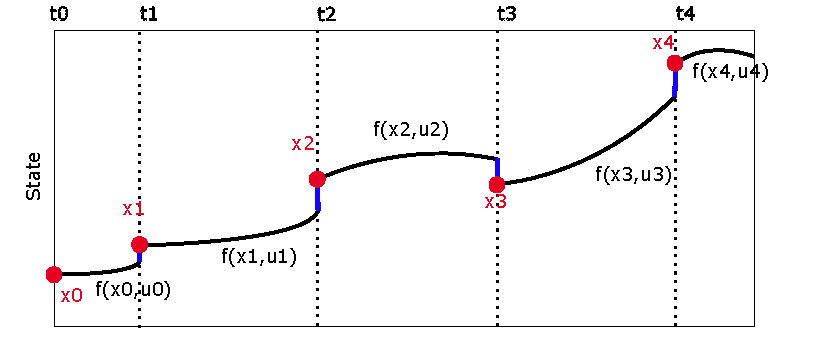
\includegraphics[width=\textwidth]{Images/MultipleShooting.pdf}
    \caption{A physically feasible trajectory is formed by "pinching" the shooting gaps close. Reproduction from \cite{gros2017Lecture}}
    \label{FIG: Shooting Gaps}
\end{figure}

\begin{equation}
    \label{EQ: RK4}
    \begin{split}
    k_1 = \quad & \textbf{f}(\bm{\theta}_{k} \ , \ \bm{\tau}_k) \\
    k_2 = \quad & \textbf{f}(\bm{\theta}_{k} + \frac{h}{2}k_1 \ , \ \bm{\tau}_k) \\
    k_3 = \quad & \textbf{f}(\bm{\theta}_{k} + \frac{h}{2}k_2 \ , \ \bm{\tau}_k) \\ 
    k_4 = \quad & \textbf{f}(\bm{\theta}_{k} + h k_3 \ , \ \bm{\tau}_k) \\ 
    \textbf{F}(\bm{\theta}_{k}, \bm{\tau}_k) = \quad & \bm{\theta}_k + \frac{h}{6} (k_1 + 2k_2 + 2k_3 + k_4)
    \end{split}
\end{equation}
Where h is the discretized time step size. With $\textbf{F}$ it is now possible to calculate $\bm{\theta}_{k+1}$ given $\bm{\theta}_k$ and $\bm{\tau}_k$
The shooting constraints are then formed as:
\begin{equation}
    \textbf{g}(\bm{\omega}) = \begin{bmatrix}
                            \overline{\bm{\theta}}_0 - \bm{\theta}_0 \\[-5pt]
                            \textbf{F}(\bm{\theta}_{0}, \bm{\tau}_0) - \bm{\theta}_1 \\[-5pt]
                            \textbf{F}(\bm{\theta}_{1}, \bm{\tau}_1) - \bm{\theta}_2 \\[-5pt]
                            \vdots \\[-5pt]
                            \textbf{F}(\bm{\theta}_{N_{p-1}}, \bm{\tau}_{N_{p-1}}) - \bm{\theta}_{N_{p}}
                             \end{bmatrix}
\end{equation}
Setting the lower and upper bounds for \textbf{g} equals to zero enforces the equality constraints and pinches the shooting gaps close. The final missing piece for the trajecotry planner
is to formulate constraints to ensure a collision free trajectory. Similarly to the shooting constraints the obstacle constraints are also placed in \textbf{g}, their
formulation is discussed in chapter \ref{CHAP: COLAV}

The theory behind constructing an \gls{NLP} in a way that a machine can understand and solve it is a topic for a whole new thesis. In this thesis CasADi, \cite{andersson2019casadi}, is used
as a framework for constructing the NLP, the NLP is solved with an \gls{IPOPT} solver, \cite{wachter2006implementation}, that comes included with CasADi. A practical
explanation of constructing and solving the NLP is the topic of chapter \ref{CHAP: Method}.

\subsubsection*{Model Predictive Control}
With the system dynamics modelled, and a control law formulated as an \gls{NLP} it is now possible to conduct trajectory planning by
selecting a discretized time step size, h, deciding how many control intervals to predict foward in time, and then solving the NLP from any initial condition
(which will still be discussed in chapter \ref{CHAP: Method}). Because the \gls{IPOPT} solver
solves for all control intervals simultaneously, its output contains the optimal trajectory as decided by the selected cost function. It also contains optimal
velocities and control inputs needed to achieve the desired state, as described by the system dynamics. However it is unrealistic to assume that the
modelled dynamics are able to perfectly represent reality, blindly following the optimal trajectory is therefor a fool's errand. This is where the
control technique \gls{MPC} comes into play. \gls{MPC} is a method in which the system is simulated from the present until the end of the control
period. The first control inputs from the solution are saved and applied to the system for it's next control interval, the rest of the solution is then
discarded and new measurements of the state of the system are taken. Using the new measurements as the new intial conditions, the process starts over;
Simulate until the end of control period, apply first control input to next control interval, discard rest of solution, redo measurements, repeat.
This grants the control system an opportunity to react and adjust to unexpected disturbances, which greatly increases robustness of the automated system.
(TODO: citation needed?)

% (TODO: REWRITE THIS, SOME PARTS MAKE LITTLE SENSE)\\
% where $\textbf{F}$ is the objective function, $\boldsymbol{\eta}(t)$ is the position and attitude trajectory of the vehicle, $\textbf{u}(t)$
% is the control input trajectory and $\textbf{L}$ is the kinematic model of the vehicle. Though the OCP can be solved
% the way it is set up in (\ref{eq:OCP description}) it is more pratical to discretize it into a ( \gls{NLP}).
% With a method called direct multiple shooting, both state and control input are defined as decision variables, the \gls{NLP} with
% $N$ control intervals is: 




\subsection{Collision Avoidance}\label{CHAP: COLAV}
\iffalse
\begin{itemize}
    \item \gls{COLREGs}
    \subitem Expected behaviour, situation classification, etc etc.
    \item \gls{dCPA} / \gls{tCPA}
    \item Other risk assessment? Situation complexity? Det er mer som inngår i "collisions avoidance" som jeg kanskje ikke dekker så veldig bra med min algoritme.
\end{itemize}
\fi

\begin{itemize}
    \item \gls{COLREGs}, cite \cite{WikisourceCOLREGS} I guess.
    \item Classification \cite{tam2010collision}.
    \item Modification \& Figur er simpelt: Courtesy of Emil Thyri.
    \item Alternative classification algorithm \cite{woerner2016multi}.
    \item dCPA og tCPA, \cite{Kufoalor2018}.
    \item My modifications to dCPA and tCPA method to get 'full coverage' of path.
    \item Static Obstacles "detection" and constraint placements
    \item Dynamic obstacles constraints.
    \item Computer vision, radar/lidar/sonar/etc. Is not a part of this thesis, see for example \cite{ruud2018lidar} for that topic.
    \item Maneuvers for avoiding collision \cite{cockcroft2012manoeuvres}
    \item No right of way, only Give Way or Stand On.
    \item cite \cite{cho2018intent} as a method for identifying intent, and a lead in to target ship prediction.
\end{itemize}

\begin{figure}
    \centering
    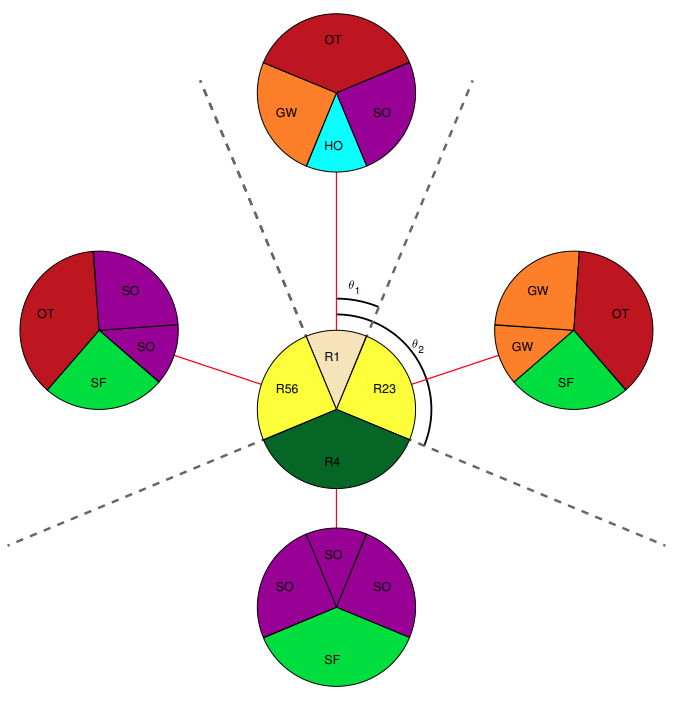
\includegraphics[height=0.35\textheight]{Images/COLREGs_assess.png}
    \caption{(TODO:ENDRE)Assigning COLREGS flag: with OS in the center we can place the TS in one of four regions. Similarly the relative bearing from TS to OS can be assigned regions with region 1 pointed directly at the OS and the rest following in a clockwise rotation.
    Courtesy of Emil Thyri.}
    \label{FIG: COLREGs Classification}
\end{figure}

\begin{figure}
    \centering
    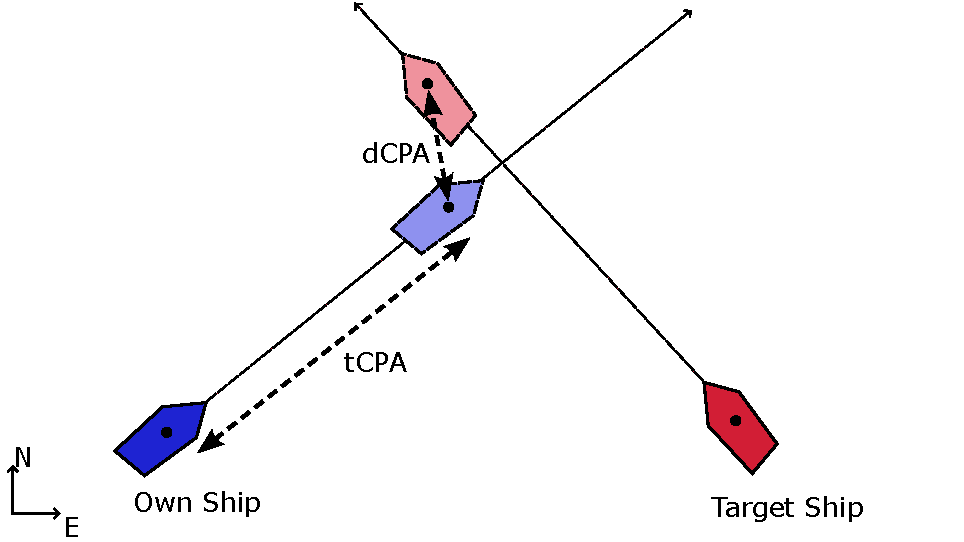
\includegraphics[width=\textwidth]{Images/shipCPA.pdf}
    \caption{Visualizing dCPA and tCPA.}
    \label{FIG: ship CPA}
\end{figure}



% \subsection{'The complete system'}
% \begin{itemize}
%     \item Vet ikke helt om dette kapittelet er nødvendig, men jeg lurer på om det er en god ide å skrive litt om nøyaktig hvor i ett fult funksjonelt
%     system jeg forventer at min algoritme passer inn. Hva de andre delene jeg ikke kommer til å skrive om har ansvar for, og hva som forventes av systemene
%     rundt mitt eget.
%     \item Hvis systemet mitt var en sort boks, hvilke inputs og outputs ville det hatt.
% \end{itemize}

% \subsection{Simulator setup}
% \begin{itemize}
%     \item liten forklaring av hvordan simulatoren funker selv om jeg ikke har laget den.
%     \item f.eks agent structs kan bli viktig.
%     \item Forklar at det er en liten forsjel på hvordan own ship agenten og andre agenter oppdateres, fører til en maksimal 'feil' på 1 meter.
% \end{itemize}

\subsection{Target Ship prediction}
--------- Genereal thoughts --------------------------
\begin{itemize}
    \item Gjenfortelling fra fordypningsprosjekt, da kalt traffic pattern
    \item Fant en annen artikkel fra Kina som skrev om nogenlunde det samme, \gls{AIS} data -\> prediksjon
    \item Skiller seg fra fordypningsprosjekt fordi det er egentlig ikke traffic pattern som er den viktige antagelsen,
    Det er heller viktig at vi antar det finnes en måte å gjette/vite hvor andre båter vil være fremover i tid.
    \item Andre metoder for target ship prediction kan være f.eks utvidelse av \gls{AIS} som 
    inkluderer autonav data for de neste 5 minuttene eller noe lignende.
    \item Disambiguate Simple and Full prediction.
\end{itemize}
---------- /General Thoughts--------------------------- 
\begin{itemize}
    \item Naval navigation is an 'active' task, always looking out for obstacles and making sure the way forward is clear.
    \item There are no lanes, instead proper conduct is dictated by \gls{COLREGs}, the rules are laid out so that different situations
    have different rules
    \item Knowing which situation you are in is half the battle, therefor the ability to predict and estiamte how encounters will happen
    is a powerful tool. Human navigators do this by experience.
    \item Autonomous vessels could also predict by experience, that would be the machine learning approach. \gls{AIS} can already provide training data.
    \item But it could be easier than that, what if \gls{AIS} data packets were expanded to send out autonav data for where a vessel intends to traverse.
    The assumption here is that vessels using autonav will correct their course when spotting a conflict. Vessels not using autonav would still be able to observe
    the indended path of other vessels and adjust their plans 'manually'.
    \item Relying on fully predicting the transit of a target vessel is fragile, relying on a few known waypoints would be much more robust.
    \item In the end the best solution would be if all vessels could fully communicate their intended path either peer to peer or through
    a centralized system. Solving conflicting paths would be done on a higher level than individual vessel.
    \item cite \cite{scholler2021trajectory} for AIS prediction.
    \item cite \cite{zhang2021collision} For mention of massive AIS data.
    \item cite ais?? har sett noen gjøre det.
    \item cite \cite{huang2020ship} to refer to current methods for target ship prediction.
\end{itemize}

\begin{figure}
    \centering
    \label{FIG: AIS lanes}
    \includegraphics[width=\textwidth]{Images/AISLanes.jpg}
    \caption{TODO: Skriv. AIS data can show common transit routes. Image courtesy of Olex AS}
\end{figure}



\newpage